\documentclass[border=4pt]{standalone}
% Preámbulo común de las figuras. Cada figura es un documento standalone
% que se compila a SVG con scripts/build_figures.sh
\usepackage[utf8]{inputenc}
\usepackage{amsmath}
\usepackage{tikz}
\usepackage[american, siunitx]{circuitikz}
\usetikzlibrary{arrows.meta,calc,decorations.pathmorphing,patterns}
\tikzset{
  >={Stealth[length=2.2mm]},
  eje/.style={->, thin},
  hilo/.style={thick},
}
% Paleta común: tonos medios legibles sobre fondo claro
\definecolor{azul}{RGB}{31,94,168}
\definecolor{rojo}{RGB}{192,57,43}
\definecolor{verde}{RGB}{39,128,73}
\definecolor{naranja}{RGB}{211,120,30}
\definecolor{morado}{RGB}{125,60,152}

\begin{document}
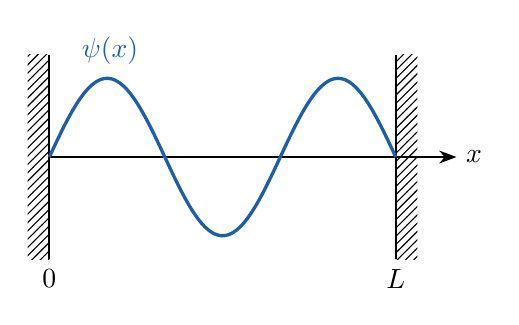
\begin{tikzpicture}[x=1.1cm, y=1.0cm]
  \fill[pattern=north east lines] (-0.25,-1.3) rectangle (0,1.3);
  \fill[pattern=north east lines] (4,-1.3) rectangle (4.25,1.3);
  \draw[thick] (0,-1.3) -- (0,1.3);
  \draw[thick] (4,-1.3) -- (4,1.3);
  \draw[eje] (0,0) -- (4.7,0) node[right]{$x$};
  \node[below] at (0,-1.3) {$0$};
  \node[below] at (4,-1.3) {$L$};
  \draw[very thick, azul] plot[domain=0:4, samples=90] (\x, {sin(deg(3*pi*\x/4))});
  \node[above, azul] at (0.7,1.05) {$\psi(x)$};
\end{tikzpicture}
\end{document}
